\documentclass[graybox]{svmult}

% -----------------------------------------------------------------------------------

% choose options for [] as required from the list % in the
% Reference Guide

\usepackage{mathptmx}       % selects Times Roman as basic font
\usepackage{helvet}         % selects Helvetica as sans-serif font
\usepackage{courier}        % selects Courier as typewriter font
\usepackage{type1cm}        % activate if the above 3 fonts are
                            % not available on your system
%
\usepackage{makeidx}         % allows index generation
\usepackage{graphicx}        % standard LaTeX graphics tool
                             % when including figure files
\usepackage{multicol}        % used for the two-column index
\usepackage[bottom]{footmisc}% places footnotes at page bottom
\usepackage{seqsplit}
\graphicspath{{Figure/}}

% -----------------------------------------------------------------------------------

\usepackage[table,xcdraw]{xcolor}
\usepackage{xcolor, soulutf8}
\newcommand{\highlight}[1]{\colorbox{yellow!50}{#1}}

\usepackage{amsmath}
% \usepackage{amssymb}         % for additional mathematical symbols
\usepackage{amsfonts}        % for sets like \mathbb{N}, \mathbb{Z}, etc.
\usepackage{bm}              % for bold symbols
\usepackage{caption}         % for controlling figure/table captions
\usepackage{float}           % to improve figure positioning


\usepackage{hyperref}
% \usepackage{apacite}
\usepackage{enumitem} 
\usepackage[small,compact]{titlesec} 
\titlespacing{\section}{0pt}{*4}{*1.5}

\usepackage{setspace}
\edef\restoreparindent{\parindent=\the\parindent\relax}
\usepackage{parskip}
\restoreparindent

% % package content table
% \usepackage{tocbasic}

% \usepackage{blindtext}

% % custom packages
\usepackage{array}
\usepackage{tabularx}
\usepackage{tabularray}
\usepackage{lineno}

\usepackage{scrextend} 
\usepackage{multirow}			% Multirow tables
\usepackage{subfig}

% to typeset URLs, URIs, and DOIs
\usepackage{url}
\usepackage{mathtools}
%  \usepackage[dvips]{graphicx}
%  \usepackage{epsfig}
 \usepackage{epsf}
% \usepackage{subfigure}
\usepackage{indentfirst}

%% The amssymb package provides various useful mathematical symbols
\renewcommand\tabularxcolumn[1]{m{#1}}
\newcommand{\itemEq}[1]{%
        \begingroup%
        \setlength{\abovedisplayskip}{0pt}%
        \setlength{\belowdisplayskip}{0pt}%
        \parbox[c]{\linewidth}{\begin{flalign}#1&&\end{flalign}}%
        \endgroup}
\newcolumntype{Y}{>{\centering\arraybackslash}X}

% see the list of further useful packages % in the Reference Guide

\makeindex             % used for the subject index
                       % please use the style svind.ist with
                       % your makeindex program

%%%%%%%%%%%%%%%%%%%%%%%%%%%%%%%%%%%%%%%%%%%%%%%%%%%%%%%%%%%%%%%%%%%%%%%%%%%%%%%%%%%%%%%%%

\begin{document}

\title*{Application of Public Key Encryption on Fuzzy Images in a Company's Security Model}
\titlerunning{Application of Public Key Encryption on Fuzzy Images in a Company's Security Model}

\author{SadNguyen, Bonten, Khoi Nguyen, Hoang Le}
\authorrunning{Bonten et al.}

\institute{Hanoi University of Science of Technology}

\maketitle

\abstract*{
    This report presents an approach to addressing the implementation of a
    security model in companies by using picture fuzzy public key encryption, with a more
    detailed focus on utilizing user biometric data as a secret key. Since biometric data is
    blurred or noisy and changes with each collection, traditional public key encryption
    models cannot be used; instead, a picture fuzzy public key encryption model must be
    employed. This study introduces the concept of picture fuzzy public key encryption
    (PFPKE), a public encryption model that accepts a portion of blurred data (a noisy version
    of the original biometric data) as a private key for decrypting the ciphertext. Unlike
    traditional public key encryption models, where the private key is typically stored on
    devices (e.g., on USB drives), the picture fuzzy public key encryption model does not
    require any device to store the private key
}

\abstract{
    This report presents an approach to addressing the implementation of a
    security model in companies by using picture fuzzy public key encryption, with a more
    detailed focus on utilizing user biometric data as a secret key. Since biometric data is
    blurred or noisy and changes with each collection, traditional public key encryption
    models cannot be used; instead, a picture fuzzy public key encryption model must be
    employed. This study introduces the concept of picture fuzzy public key encryption
    (PFPKE), a public encryption model that accepts a portion of blurred data (a noisy version
    of the original biometric data) as a private key for decrypting the ciphertext. Unlike
    traditional public key encryption models, where the private key is typically stored on
    devices (e.g., on USB drives), the picture fuzzy public key encryption model does not
    require any device to store the private key
}

\keywords{Picture fuzzy public key encryption, fuzzy data, biometrics}

\section{Introduction}
In traditional security models within companies using public key infrastructure, each employee must have a public-private key pair. If an employee receives an \allowbreak encrypted message, it means the message has been encrypted using that employee's public key, and they will decrypt it with their private key. The most important aspect for the employee is to keep their private key secure, as a leak of this key would compromise the system's security. A widely accepted method is to store the private key on a physical device like a smart card or USB drive and require the employee to remember a password to activate it
(Ellison, C., Schneier, B. 2000).
%  \cite{Ellison2000}.
An ideal approach is to use biometric data (e.g., fingerprints or iris patterns)
(Connaughton, R., Bowyer, K.W., Flynn, P.J. 2007)
% \cite{Connaughton2007}
as a private key since biometric data is unique to each individual, providing a convenient and secure way to serve as a private key for users. However, biometric data can be blurry or noisy and may change every time it is captured, making it unsuitable for use as a private key in traditional public key encryption schemes.
To address this issue, this paper introduces the concept of fuzzy signatures
(Takahashi, K., Matsuda, T., Murakami, T., Hanaoka, G., Nishigaki 2015)
% \cite{Takahashi2015}
,which use biometric data as a private key without requiring any assistance
(Dodis, Y., Ostrovsky, R., Reyzin, L., Smith, A.D. 2008)
% \cite{Dodis2008}
. Thus, it applies public key cryptography with fuzzy images
(Son, LH, Viet, PV, \& Hai, PV 2016)
% \cite{Son2016}
in internal company security models utilizing biometrics.

\section{Symbols and definitions}
\begin{enumerate}[label=(\roman*), itemsep=1em]
    \item Let \( \mathbb{N} \), \( \mathbb{Z} \), and \( \mathbb{R} \) denote the sets of natural numbers, integers, and real numbers, respectively. If \( n \in \mathbb{N} \), let \( [n] := \{1,\, \ldots,\, n\} \). If \( a \in \mathbb{R} \), then \( \lfloor a \rceil \) denotes the nearest integer to \( a \). Additionally, if \( a = (a_1,\, a_2,\, \ldots) \), let \( \lfloor a \rceil := (\lfloor a_1 \rceil,\, \lfloor a_2 \rceil,\, \ldots) \).
    \item The notation \( x \leftarrow y \) denotes that \( y \) is assigned to \( x \). If \( S \) is a finite set, \( |S| \) represents its size, and \( x \leftarrow_{{R}}   S \) means that \( x \) is chosen randomly from \( S \). If \( \varPhi \) is a distribution over some set, \( x \leftarrow_R \varPhi \) denotes that \( x \) is chosen according to distribution \( \varPhi \). Let \( f: D \rightarrow R \) be a function and \( y \in R \) a value; \( { f^{-1}(y) } \) represents the set of pre-images of \( y \) under \( f \), i.e., \( { f^{-1}(y) = \{x \in D \mid f(x) = y\} } \). If \( x \) and \( y \) are bitstrings, then \( |x| \) denotes the bit length of \( x \), and \( (x || y) \) represents the concatenation of \( x \) and \( y \).
    \item A function \( f(.): \mathbb{N} \rightarrow [0, 1] \) is called negligible if for every positive polynomial \( p(.) \) and every sufficiently large \( \lambda \) then \( f(\lambda) < \dfrac{1}{p(\lambda)} \).
    \item How to set the open key: \\
          1 open key setting \( \mathcal{F} \) includes \( ((d, X), t, \mathcal{X}  , \varPhi, \epsilon) \) with \( (d, X) \) being the \allowbreak spatial data with \( X \) being the space containing the values of the fuzzy set of the \allowbreak picture \( A \) and \( d : X^2 \to \mathbb{R} \) being the corresponding distance function. \( t \in \mathbb{R} \) is the \allowbreak threshold value determined by the security parameter \( \lambda \), \( \mathcal{X} \) is the \allowbreak distribution of the fuzzy data on \( X \), \( \varPhi \) is the error distribution and \( \epsilon \in [0,1] \) is an error \allowbreak parameter representing the false rejection rate. The False Acceptance Rate (FAR) and False Rejection Rate (FRR) are determined based on the threshold value \( t \).\\[6pt]
          \textbf{Requirement}: \( \text{FAR} := \Pr[x,\, x' \leftarrow_{{R}} {\mathcal{X}} : d(x,\, x') < t] \) is negligible in the \allowbreak security parameter  \( \lambda \). Also for all fuzzy data parts of \( x \in {X} \), \( \text{FRR} := \Pr[e \leftarrow_{{R}} \varPhi : \mathrm{d}(x, \, x + e) \geq t] \leq \epsilon \)
    \item The definition of picture fuzzy set (PFS) is an extension of fuzzy set and \allowbreak intuitionistic fuzzy set. Picture fuzzy set is based on a complete model in \allowbreak situations where we have human opinions: yes, no, neutral. \\[6pt]
          Given a background set \( X = \{x_1, x_2, \dots, x_n \} \), a picture fuzzy set \( A \) on \( X \) is \allowbreak defined by
          \[
              A = \left\{ \langle x,\, \mu_A(x),\, \eta_A(x),\, \nu_A(x) \rangle \mid x \in X \right\}
          \]

          Where:
          \begin{align*}
              \mu_A  & : X \to [0, 1] \quad \text{is a positive function} \\[6pt]
              \eta_A & : X \to [0, 1] \quad \text{is a neutral function}  \\[6pt]
              \nu_A  & : X \to [0, 1] \quad \text{is a negative function}
          \end{align*}

          Satisfy the condition:
          \[
              \mu_A(x) + \eta_A(x) + \nu_A(x) < 1 \quad \forall x \in X
          \]

          Apply the \( L- R \) fuzzy number formula to calculate \( \mu(x) = \langle b, c \rangle \), where \( b \) is the average value in set \( X \), and \( c \) is the maximum value in set \( X \):
          \[
              \mu(x) = \begin{cases}
                  0                & \text{if } x \leq c     \\
                  \dfrac{x-b}{c-b} & \text{if } b < x \leq c
              \end{cases}
          \]

          Apply the triangular fuzzy number formula to calculate \( \eta(x) = \langle a, b, c \rangle \), where \( b \) is the average value in the set \( X \):
          \begin{align*}
              a       & = \dfrac{b + \min(X)}{2}                                          \\[6pt]
              c       & = \dfrac{b + \max(X)}{2}                                          \\[6pt]
              \eta(x) & = \begin{cases}
                              0                & \text{if } x \geq c \text{ or } x < a \\
                              \dfrac{c-x}{c-b} & \text{if } b \leq x < c               \\[6pt]
                              \dfrac{x-a}{b-a} & \text{if } a \leq x < b
                          \end{cases}
          \end{align*}


          Apply the \( L - R \) fuzzy number formula to calculate \( \nu(x) = \langle a, b \rangle \), where \( b \) is the average value in set \( X \), and \( a \) is the minimum value in set \( X \):
          \[
              \nu(x) = \begin{cases}
                  0                & \text{if } x \geq a     \\
                  \dfrac{b-x}{b-a} & \text{if } a \leq x < b
              \end{cases}
          \]

\end{enumerate}


\begin{figure}[H]
    \centering
    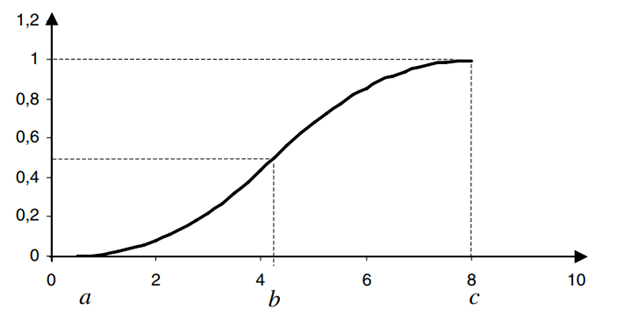
\includegraphics[width=\textwidth, keepaspectratio]{Figure1.png} % Adjust the width or use \textwidth for relative size
    \caption{Membership functions applied to high level of security of fuzzy sets of pictures}
    \label{fig:membership-functions-security}
\end{figure}

\section{Famework and security model of public key cryptography of watermark}
\subsection*{A. Framework of Public Key Cryptography for Watermark}

The public key cryptography scheme consists of the following six algorithms: Key Extraction, Setup Algorithm, Key Generation Algorithm, Encrypt Algorithm, and Decrypt Algorithm:

\begin{itemize}
    \item \textbf{Extract the fuzzy picture (Bio)}
          \[
              \{ \langle x,\, \mu_A(x),\, \eta_A(x),\, \nu_A(x) \rangle \mid x \in X \}
          \]
          When entering the user's biometric information, the algorithm will output the fuzzy picture data.

    \item \textbf{Set} \( (1^\lambda) \to par  \): when entering the security parameter \( \lambda \), this algorithm will output the public parameter \(  par \), including the fuzzy key setting
          \[
              \mathcal{F} = ((d, \, X), \, t, \, X, \, \varPhi, \, \epsilon)
          \]

    \item \textbf{KeyGen} \( (par ,\, x) \to \text{pk}_f \): when entering the public parameter \(  par \) and the fuzzy picture data of \( x \in X \), this algorithm outputs the public key \( \text{pk}_f \).

    \item \textbf{Encryption} \( (par ,\, \text{pk}_f,\, M) \to \text{CT} \): When entering the public parameter \(  par \), the public key \( \text{pk}_f \) and the message \( M \) (in the message space), this algorithm outputs the ciphertext \( \text{CT} \).

    \item \textbf{Extract the fuzzy picture (Bio)}
          \[
              \{ \langle x', \mu_A(x'), \eta_A(x'), \nu_A(x') \rangle \mid x' \in X \}
          \]
          When entering the user's biometric information, the algorithm will output the fuzzy picture data.

    \item \textbf{Decrypt} \( (par , \text{pk}_f, x', \text{CT}) \to M/\perp \): When entering the public parameter \(  par \), the public key \( \text{pk}_f \), the fuzzy picture data of \( x' \in X \), and the ciphertext \text{CT}, this algorithm outputs the message \( M \) or the error symbol \( \perp \).

\end{itemize}

We say that the public key encryption scheme of a fuzzy picture with the fuzzy key setting \( \mathcal{F} \) is correct, meaning that for every security parameter \( \lambda \in \mathbb{N} \) with all fuzzy picture data of \( x, x' \in X \) such that \( \mathrm{d}(x, x') < t \), for all messages \( M \) in the \allowbreak message space, if:
\begin{align*}
    par         & \leftarrow \text{Set}(1^\lambda)                    \\[6pt]
    \text{pk}_f & \leftarrow \text{KeyGen}(par ,\, x)                 \\[6pt]
    \text{CT}   & \leftarrow \text{Encrypt}(par ,\, \text{pk}_f,\, M)
\end{align*}

we get:
\[
    \text{Decrypt}(par ,\, \text{pk}_f,\, x',\, \text{CT}) = M
\]

\subsection*{B. Security Model}

Similar to the security definition of a public key cryptography scheme, a fuzzy public key cryptography scheme is required to be indistinguishable under universal faults of the fuzzy key setting \( \mathcal{F} \).
A fuzzy public key cryptography scheme in fuzzy key setting \( \mathcal{F} \) is said to be indistinguishable under chosen ciphertext attacks (IND-CCA security) if for any adversary \( \mathcal{A} \) we have an advantage function given by:

\begin{equation*}
    Adv\begin{array}{c}
        ind-cca                  \\
        \text{FPKE}, \mathcal{A} \\
    \end{array} (\lambda)
    =
    Pr\left[b'= b \left| \begin{array}{c}
            par  \leftarrow Init(1^\lambda)                                                         \\
            x^* \leftarrow_{R} \mathcal{X}, \, b \leftarrow \{0, 1 \}                               \\
            pk^*_f \leftarrow KeyGen(par , \, x^*)                                                  \\

            (M_{0}, \, M_{1}, \, \text{state}) \leftarrow \mathcal{A}^{O_{Dec(.)}}(par , \, pk^*_f) \\
            CT^* \leftarrow Encrypt(par , \, pk^*_f, \, M)                                          \\
            b' \leftarrow \mathcal{A}^{O_{Dec(.)}}(par  , \, pk^*_f, \, M_0, \, M_1, \, \text{state}, \, CT^*)
        \end{array} \right. \right] - \frac{1}{2}
\end{equation*}
This is negligible in the security parameter \( \lambda \), with \( |M_0| = |M_1| \) and \( O_{\text{DEC}(.)} \) \allowbreak being the decryption guess, taking the public parameter \(  par \), the public key \( \text{pk}_f^* \), a \allowbreak fragment of the watermark data \( x^* \), and a fragment of the ciphertext \( \text{CT} \) as input, and \allowbreak outputting the message \( M \leftarrow \text{Decrypt}(par ,\, \text{pk}_f^*,\, x^*,\, \text{CT}) \).


\section{Construct algorithm for fuzzy public key encryption}
\subsection*{- Encryption Algorithm}
\begin{figure}[H]
    \centering
    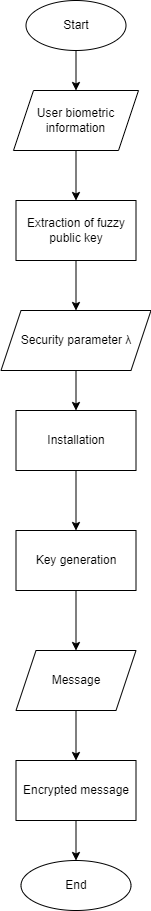
\includegraphics[width=0.3\textwidth, keepaspectratio]{Encryption.png} % Adjust the width or use \textwidth for relative size
    \label{fig:encryption-algorithm}
\end{figure}


Example of the Encryption Algorithm:
\begin{enumerate}[itemsep=1em]
    \item First, the algorithm will perform the extraction of the biometric information of the user that has been encoded into a vector \( x = (5, 7, \dots, 1) \).
    \item Then, it will extract the information of the fuzzy public key \( A = \langle 0.75, 0.1, 0.15 \rangle \).
    \item After that, choose \( \lambda \) as a random number in the range \( \{0, \, 2^{64} - 1\} \) as the input security parameter.
    \item Execute the installation algorithm to obtain the output public parameter:\\
          par =
          \seqsplit{\textquotedblleft MFwwDQYJKoZIhvcNAQEBBQADSwAwSAJBAJQVu6lHAEtia3xc8fCEKd9dpt0jGt7FSiMz\textquotedblright}


    \item With \( par \) and fuzzy public key data obtained above through the key generation algorithm, the output public key \\ \( pk_f = (pk, \, c) \) =
          \seqsplit{(MFwwDQYJKoZIhvcNAQEBBQADSwAwSAJBAKD/RZvqG4ocFdsCpVpUbgrlYlEumD9qebAIVm3gv1Y6XN7w6jf2B4V9soP9jbXcmwEDy/N6xognyuqKAEB81JUCAwEAAQ==, \, MFwwDQYJKoZIhvcNAQEBBQADSwAwSAJBAKNQ0UmtSE2dD6Mbx0Vd8GWcTYvqPJNTqyg7xtJAYWWGPmjScKH1VUZw0lIRve3mtlLoxa7mRntUm6iw94ZSCXcCAwEAAQ).}

    \item Input the message to be encrypted \\ \( M = \text{\textquotedblleft PUBLIC ENCRYPTION OF FUZZY PUBLIC KEY\textquotedblright} \) into the algorithm. From the message to be encrypted and the key obtained above through the \allowbreak encryption algorithm, we obtain the ciphertext:\\ \( CT \)
          =  \seqsplit{\textquotedblleft exhxWbrXSm7huDc/4LkAHnmk3i91K1FDBqUwpk01gLR0pY8Ow/SQe3xPLpdkSpoTLwm/T3KqI0qGs8HehzXHHw==\textquotedblright}.
\end{enumerate}

\subsection*{- Decryption Algorithm}
\begin{figure}[H]
    \centering
    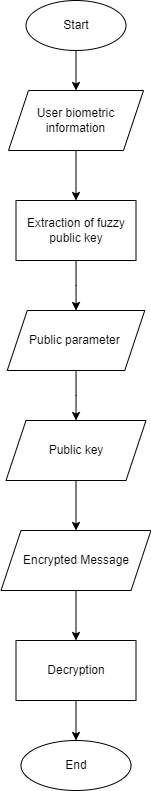
\includegraphics[width=0.35\textwidth, keepaspectratio]{Decryption.png} % Adjust the width or use \textwidth for relative size
    \label{fig:decryption-algorithm}
\end{figure}

Example of the Decryption Algorithm:
\begin{enumerate}[itemsep=1em]
    \item First, the algorithm will perform the extraction of the biometric information of the user that has been encoded into a vector \( x' = (5,\, 6, \, \dots, \, 1) \).
    \item Then, it will extract the information of the fuzzy public key. The output will be the data of the fuzzy public key \( A = \langle 0.74,\, 0.1,\, 0.15 \rangle \).
    \item With the input parameters, including the fuzzy public key, the public parameter:
          \\[6pt] \( par \) = \seqsplit{\textquotedblleft MFwwDQYJKoZIhvcNAQEBBQADSwAwSAJBAJQVu6lHAEtia3xc8fCEKd9dpt0jGt7FSiMz\textquotedblright},
          public key:
          \\[6pt] \( pk_f \) = \seqsplit{(MFwwDQYJKoZIhvcNAQEBBQADSwAwSAJBAKD/RZvqG4ocFdsCpVpUbgrlYlEu mD9qebAIVm3gv1Y6XN7w6jf2B4V9soP9jbXcmwEDy/N6xognyuqKAEB81JUCAwEAAQ==, MFwwDQYJKoZIhvcNAQEBBQADSwAwSAJBAKNQ0UmtSE2dD6Mbx0Vd8GWcTYvqPJ NTqyg7xtJAYWWGPmjScKH1VUZw0lIRve3mtlLoxa7mRntUm6iw94ZSCXcCAwEAAQ)},
          \\[6pt] and the code\\ \( CT \) = \seqsplit{\textquotedblleft exhxWbrXSm7huDc/4LkAHnmk3i91K1FDBqUwpk01gLR0pY8Ow/SQe3xPLpdkSpoTL wm/T3KqI0qGs8HehzXHHw==\textquotedblright.}
    \item After the decryption algorithm, we obtain:
          \( M \) = \textquotedblleft PUBLIC KEY ENCRYPTION OF THE FUZZY PUBLIC KEY\textquotedblright.
\end{enumerate}

\subsection*{- Detailed Implementation of the Algorithm}
Install the fuzzy key \( \mathcal{F} = ((d, X), t, \mathcal{X}, \varPhi, \epsilon) \). The Public Fuzzy Public Key \allowbreak Encryption (PFPKE) includes extracting the fuzzy representation, installation, \allowbreak Keygen, key code, and decryption, ensuring IND-CCA security, with \( K \) being the space of private keys that determine the key characteristics and homomorphism.

Assume that \( S = (\text{S.Setup},\, \text{S.Sketch}, \text{S.DiffRec}) \) is the probabilistic algorithm for installing the fuzzy key \( \mathcal{F} \), and \( \text{Sig} = (\text{Sig.KeyGen},\, \text{Sig.Sign},\, \text{Sig.Verify}) \) is the \allowbreak one-time signature algorithm.

The public-key cryptographic scheme of the fuzzy representation (PFPKE) is linked to the installation of the fuzzy key \( \mathcal{F} \), including the following steps:

\begin{enumerate}
    \item \textbf{Extract the fuzzy representation}: This step takes the biometric information of the user as input. The output is the fuzzy representation data:
          \[
              \text{Gen(Bio)} = \left\{ \langle x,\, \mu_A(x),\, \eta_A(x),\, \nu_A(x) \rangle \mid x \in X \right\}.
          \]

    \item \textbf{Installation}: The security parameter \( \lambda \) is taken as input. It defines the \allowbreak installation of the fuzzy key \( \mathcal{F} = ((d,\, X),\, t,\, \mathcal{X},\, \varPhi,\, \epsilon) \). The public parameter \(  par \) is \allowbreak obtained:
          \[
              par_{pke} \leftarrow_R S.\text{Setup}(1^\lambda), \quad par_S \leftarrow_R S.\text{Setup}(\kappa, +).
          \]
          The final public parameter is:
          \[
              par  = (par_{pke},\, par_S,\, \mathcal{F}).
          \]

    \item \textbf{KeyGen}: Takes the public parameter \(  par \) and a part of the fuzzy representation data of \( x \) as input. It parses \( par  = (par_{pke}, par_S) \), then runs:
          \[
              sk \leftarrow_R \kappa, \quad pk \leftarrow \text{KeyGen}(par_{pke}, \, sk), \quad c \leftarrow_R S.\text{Sketch}(par_S, \, sk, \, x).
          \]
          The output is the public key:
          \[
              pk_f = (pk,\, c)
          \]

    \item \textbf{Encryption}: Takes the public parameters \(  par \), the public key \( pk_f \), and the \allowbreak message \( M \) as input. It parses \( par  = ( par_{pke}, par_S) \) and \( pk_f = (pk, \, c) \). The \allowbreak signature key generation algorithm is run:
          \[
              ssk \leftarrow \text{Sig.KeyGen}(),
          \]
          generating the signing key $ssk$ and verification key $svk$. The ciphertext $CT$ is obtained by running:
          \[
              CT \leftarrow_R \text{Encoding}(par_{pke}, \, pk, \, svk, \, M).
          \]
          The signature $\sigma$ is created with the signing key $ssk$ on $CT$, and the final output is the encoded message:
          \[
              CT = (svk, \, CT, \, \sigma).
          \]

    \item \textbf{Extract fuzzy representation}: This step takes the user's biometric information as input. The output is the fuzzy representation data:
          \[
              \text{Gen}(\text{Bio}) = \left\{ \langle x', \, \mu_A(x'), \, \eta_A(x'), \, \nu_A(x') \rangle \mid x' \in X \right\}.
          \]

    \item \textbf{Decryption}: Takes the public parameters \(  par \), the public key \( pk_f \), the fuzzy representation data of \( x' \in X \), and the encoded message \( CT \) as input. It parses \( par  = (par_{pke}, par_S) \), \( pk_f = (pk, \, c) \), and \( CT = (svk, \, CT, \, \sigma) \). If \( \sigma \) is the signature on \( CT \) with respect to the public key \( svk \), it will run:
          \begin{align*}
              sk' & \leftarrow_R \kappa                              \\
              pk' & \leftarrow \text{KeyGen'}(par_{pke}, sk')        \\
              c'  & \leftarrow S.\text{Sketch}(par_S, \, sk', \, x')
          \end{align*}

          The difference key \( \Delta sk \) is obtained by:
          \[
              \Delta sk \leftarrow S.\text{DiffRec}(par_S, \, c, \, c0).
          \]
          Finally, decryption proceeds as:
          \[
              M \leftarrow \text{Decoding}(par_{pke}, \, \Delta sk, \, CT, \, pk', \, sk'),
          \]
          and the output is the message \( M \).
\end{enumerate}

\section{Some additional properties}
For the public key encryption scheme used to construct the public key encoding of the fuzzy representation, it is necessary to define some additional properties:

\subsection{Key Determination Scheme}

The decision key is the KeyGen algorithm that first randomly selects a key \( sk_{pke} \) (from the secret key space) and calculates the corresponding public key \( pk_{pke} \) \allowbreak (determined by the secret key \( {sk}_{pke} \)) during the key generation process. Formally, a public-key cryptographic scheme is a Key Determination Scheme if the public \allowbreak parameter \( {par}_{pke} \) is generated by a specified set algorithm, specifying the private key space \( \kappa_{pke} \), and there exists a specified algorithm KeyGen' such that the \allowbreak algorithm to generate the key KeyGen can be defined as \( \text{KeyGen}(par_{pke}) \):
\[
    sk_{pke} \leftarrow_R \kappa_{pke}; \quad pk_{pke} \leftarrow \text{KeyGen}'(par_{pke}, \, sk_{pke}); \quad \text{Return } (sk_{pke}, \, pk_{pke}).
\]

\subsection{Homomorphism}

The public key encryption scheme is homomorphic if it satisfies the following conditions:
\begin{itemize}
    \item For the public parameters \( par_{pke} \) generated by the setup algorithm, there is an abelian group \( (\kappa_{pke}, +) \) associated with the private key space \( \kappa_{pke} \).
    \item There exists a deterministic algorithm denoted as \( \kappa_{{pk}_{pke}} \) that takes the public parameters \( par_{pke} \), the public key \( pk_{pke} \), and an input \(\Delta{sk} \in \kappa_{pke} \), and outputs a shifted public key \({pk}_{pke}'\). For every \( {par}_{pke} \) in the setup algorithm:
          \[
              \text{KeyGen}'( {par}_{pke}, \, {sk}_{pke} + \Delta{sk}) = M_{{pk}_{pke}} ({par}_{pke}, \, \text{KeyGen}'({par}_{pke}, \, {sk}_{pke}, \, \Delta{sk}))
          \]

    \item There exists an algorithm that determines \( M_{en} \), taking the public parameters \( par_{pke} \), public key \( pk_{pke} \), ciphertext \( CT \), and shifted private key \( \Delta sk \in \kappa_{pke} \) as input, and outputs the shifted ciphertext message.
\end{itemize}

\section{Conclusion}
In the traditional method, messages encrypted using public key schemes rely on protecting the privacy of the user's private key by storing it in a physical device, such as a USB token carried by the user. However, it is not always practical for the user to keep the device with them at all times. To solve this problem, using individual biometric data as the private key is a reasonable alternative.

However, biometric data can change every time it is collected, making it \allowbreak unsuitable for direct use as a private key. In this paper, the concept of public key cryptography with fuzzy data is introduced, where a part of the biometric data can be used as the private key to decrypt ciphertexts without requiring any additional information.

Compared to traditional public key encryption, the primary advantage of fuzzy public key encryption is that it does not require the user to carry any memory device or password to function as a private key. When using fuzzy public key encryption, attention should be paid to the value of the fuzzy set in the neutral degree, as these unclear points in system access allow potential vulnerabilities where hackers could access the system.

\section*{Acknowledgments}
Acknowledgments section


% References
\bibliographystyle{plain}
\bibliography{references}


\end{document}